% \documentclass[ba,preprint]{imsart}% use this for supplement article
\documentclass[ba]{imsart}

%% Packages
\RequirePackage{amsthm,amsmath,amsfonts,amssymb}
\RequirePackage[numbers]{natbib}
%\RequirePackage[authoryear]{natbib}%% uncomment this for author-year citations
\RequirePackage[colorlinks,citecolor=blue,urlcolor=blue,backref=page,backref=page]{hyperref}
\RequirePackage{graphicx}


%%%%%%%%%%%packages added by Spencer%%%%%%%%%%%%%
\usepackage{booktabs} %for the table in the analysis section
\usepackage{enumerate} %for the short algorithm
\usepackage{subfigure} %for making plots with multiple images
\usepackage{tabularx} %for the spacing in tabular
%%%%%%%%%%%%%%%%%%%%%%%%%%%%%%%%%%%%%%%%%%%%%%%%%

\pubyear{2024}
\arxiv{2010.00000}
\volume{TBA}
\issue{TBA}
\firstpage{1}
\lastpage{1}

\startlocaldefs
%%%%%%%%%%%%%%%%%%%%%%%%%%%%%%%%%%%%%%%%%%%%%%
%%                                          %%
%% Uncomment next line to change            %%
%% the type of equation numbering           %%
%%                                          %%
%%%%%%%%%%%%%%%%%%%%%%%%%%%%%%%%%%%%%%%%%%%%%%
%\numberwithin{equation}{section}
%%%%%%%%%%%%%%%%%%%%%%%%%%%%%%%%%%%%%%%%%%%%%%
%%                                          %%
%% For Axiom, Claim, Corollary, Hypothesis, %%
%% Lemma, Theorem, Proposition              %%
%% use \theoremstyle{plain}                 %%
%%                                          %%
%%%%%%%%%%%%%%%%%%%%%%%%%%%%%%%%%%%%%%%%%%%%%%
\theoremstyle{plain}
\newtheorem{axiom}{Axiom}
\newtheorem{claim}[axiom]{Claim}
\newtheorem{theorem}{Theorem}[section]
\newtheorem{lemma}[theorem]{Lemma}
%%%%%%%%%%%%%%%%%%%%%%%%%%%%%%%%%%%%%%%%%%%%%%
%%                                          %%
%% For Assumption, Definition, Example,     %%
%% Notation, Property, Remark, Fact         %%
%% use \theoremstyle{definition}            %%
%%                                          %%
%%%%%%%%%%%%%%%%%%%%%%%%%%%%%%%%%%%%%%%%%%%%%%
\theoremstyle{definition}
\newtheorem{definition}[theorem]{Definition}
\newtheorem*{example}{Example}
\newtheorem*{fact}{Fact}
%%%%%%%%%%%%%%%%%%%%%%%%%%%%%%%%%%%%%%%%%%%%%%
%%                                          %%
%% For Case use \theoremstyle{remark}       %%
%%                                          %%
%%%%%%%%%%%%%%%%%%%%%%%%%%%%%%%%%%%%%%%%%%%%%%
\theoremstyle{remark}
\newtheorem{case}{Case}
%%%%%%%%%%%%%%%%%%%%%%%%%%%%%%%%%%%%%%%%%%%%%%
%% Please put your definitions here:        %%
%%%%%%%%%%%%%%%%%%%%%%%%%%%%%%%%%%%%%%%%%%%%%%
\endlocaldefs

\begin{document}


\begin{supplement}
\renewcommand{\thesection}{\Alph{section}}

\section{Additional plots for ILI \& Hospitalization data for select regions,
         results from simulation study, and 2023-24 flu analysis}

Figure \ref{fig:ili_vs_week} shows ILI data from five states and the District of Columbia, locations which received particular attention in \cite{osthus2021multiscale}. The plots include the ILI data for all seasons from 2010 to 2023 in grey, and the black line is the per week ILI average over seasons. The patterns in the individual states are similar to the national level plots in that the ILI rises in the fall and winter until it peaks and descends as the spring and summer progress. For these locations ILI regularly peaks, either locally or globally, at or near week 22. 

 \begin{figure}[hbt!]
    \centering
    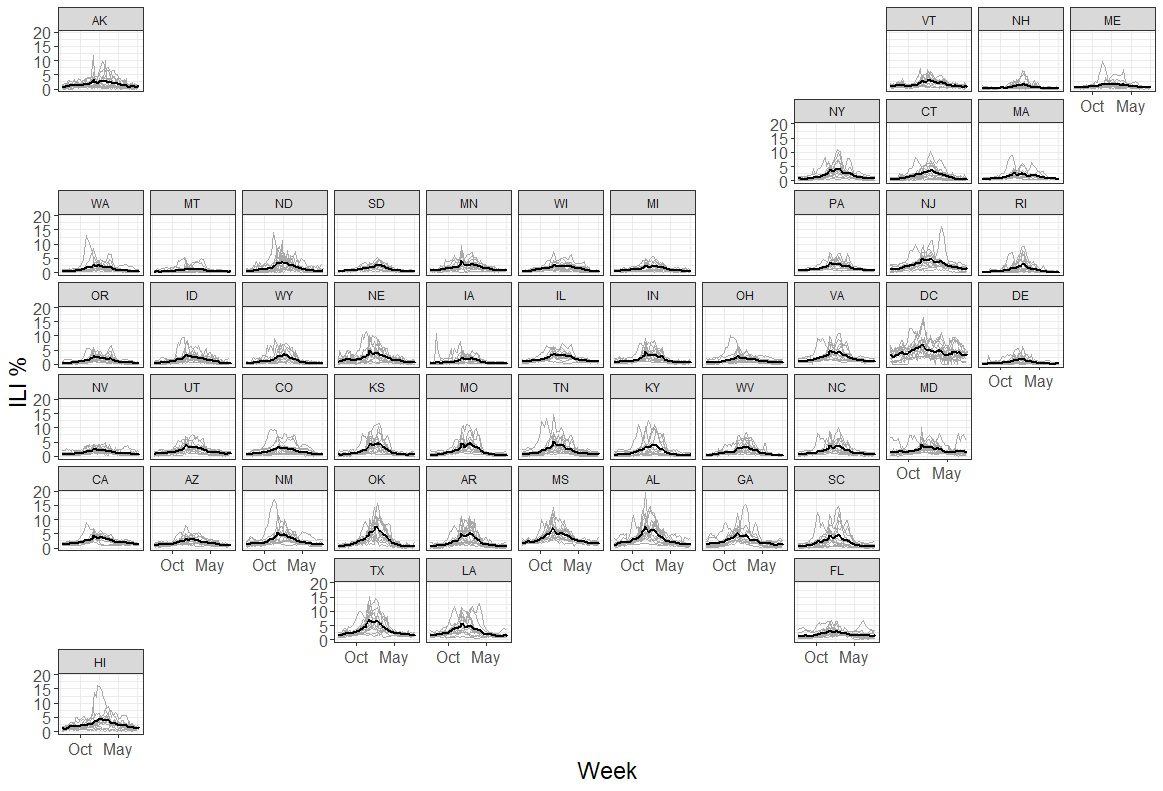
\includegraphics[scale=.7]{Images/ili_vs_week.png}
    \caption{Percentage of outpatient visits with an influenza-like illness (ILI) in five different states and the District of Columbia for seasons 2010 to 2023. Week 1 is the first week of August of the year the flu season begins and the last week of the season is the last week of July of the following year.
     Plots include lines for ILI\% from the 2010 flu season to 2023 (grey) and for the weekly ILI averaged over all seasons (black).}
    \label{fig:ili_vs_week}
\end{figure}


Figure \ref{fig:hosp_vs_week} shows the 2022 and 2023 weekly hospitalizations for the same states from \ref{fig:ili_vs_week}. Similar to the national data, the peak in 2022 came early compared to the peak of 2023. Comparing figures \ref{fig:ili_vs_week} and \ref{fig:hosp_vs_week} shows that ILI and hospitalizations share the similar pattern of increasing to a peak in the winter and decreasing thereafter. 

\begin{figure}[hbt!]
    \centering
    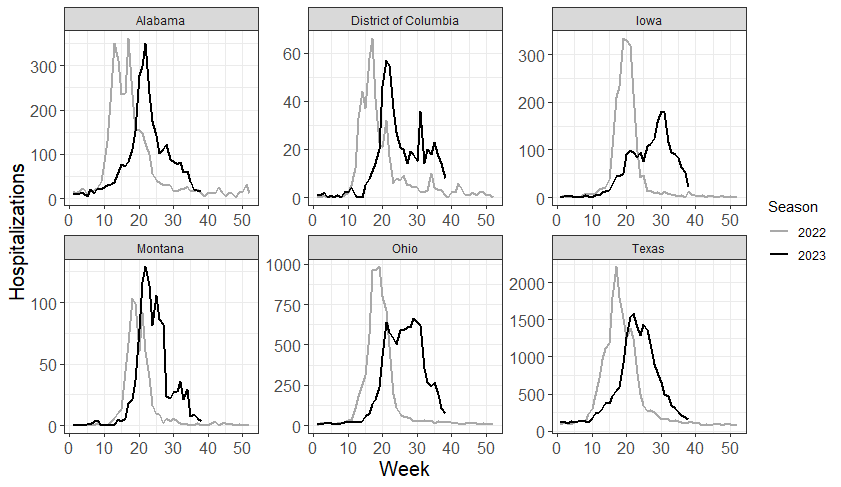
\includegraphics[scale=.65]{Images/hosp_vs_week.png}
    \caption{Weekly hospitalization counts for five states and DC for the 2022 (grey) and 2023 (black) flu seasons}
    \label{fig:hosp_vs_week}
\end{figure}





% Figure \ref{fig:ili_vs_hosp} shows scatter plots with ILI\% on the $x$-axes and hospitalizations on the $y$-axes, revealing a positive somewhat linear relationship between the two variables. This relationship motivates the forecast models outlined in the next section. 
% 
% \begin{figure}[hbt!]
%     \centering
%     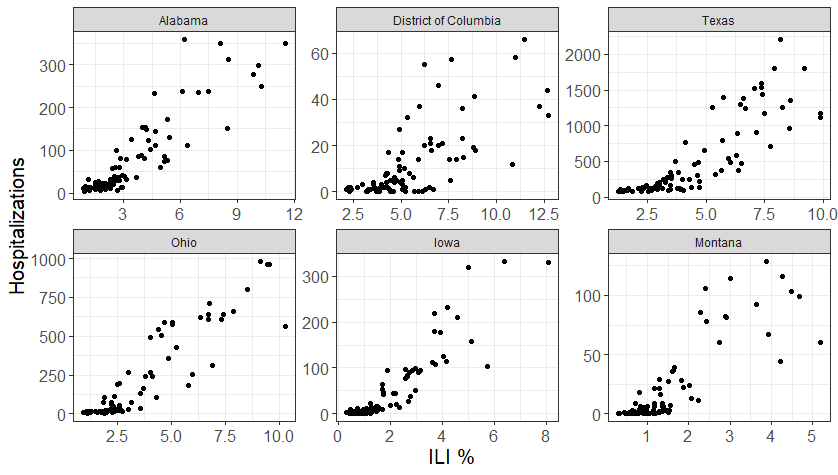
\includegraphics[scale=.6]{Images/ili_vs_hosp.png}
%     \caption{Weekly flu confirmed hospitalization counts ($y$-axis) for five states and the District of Columbia for the 2022 and 2023 flu seasons plotted against ILI\% ($x$-axis)}
%     \label{fig:ili_vs_hosp}
% \end{figure}




% \section{Additional results plots from simulation study}


Figures \ref{fig:overall_scores} - \ref{fig:logs_by_season} show boxplots of the CRPS and LogS for the four models. Figure \ref{fig:overall_scores} shows that the variation of overall CRPS is smallest for the ASG models and larger for the SIR models. The median scores for the SIR models also appears slightly higher than for the ASG models. 
When faceted by season in figure \ref{fig:crps_by_season}, the boxplots of the CRPS often show the same pattern for ASG and SIR models but not always. For example, the bulk of CRPS values for the SIRD model in 2019 appears to have smaller variation than the other models.
The LogS plots show similar results to the CRPS plots, though there are some differences. For example, SIRD in figure \ref{fig:logs_by_season} tends to show smaller LogS variation relative to the other three models than is seen by the CRPS of SIRD in figure \ref{fig:crps_by_season}.

\begin{figure}[hbt!]
\centering
% \begin{subfigure}{.5\textwidth}
  \centering
  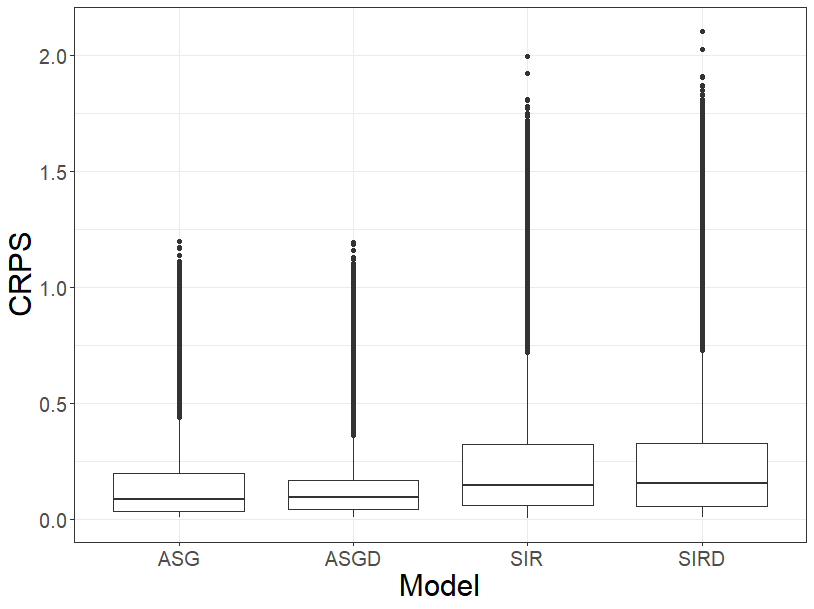
\includegraphics[scale=.3]{Images/overall_crps.png}
    % \caption{Boxplots of CRPS for the four ILI models over all seasons, weeks, and horizons in the simulation study}
% \end{subfigure}%
% \begin{subfigure}{.5\textwidth}
  \centering
  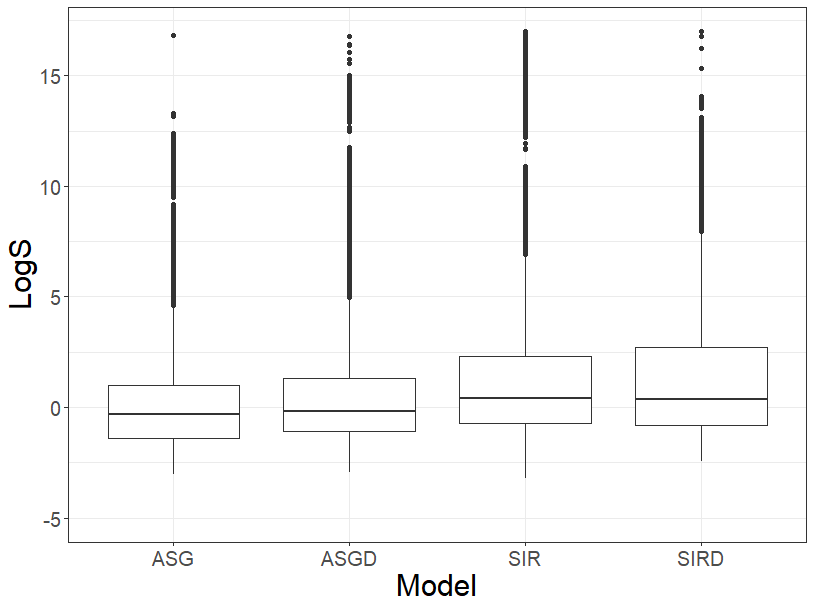
\includegraphics[scale=.3]{Images/overall_logs.png}
    % \caption{Boxplots of LogS for the four ILI models over all seasons, weeks, and horizons in the simulation study}}
% \end{subfigure}
\caption{Boxplots of the continuous ranked probability score (CRPS) (left) and logarithmic score (LogS) (right) for the four ILI models over all seasons, weeks, and horizons in the simulation study}
\label{fig:overall_scores}
\end{figure}



\begin{figure}[hbt!]
    \centering
    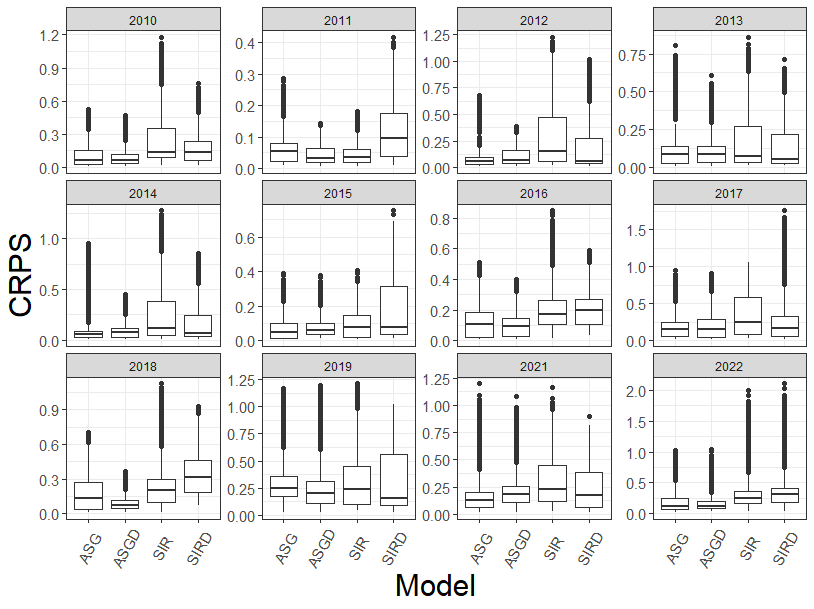
\includegraphics[scale=.5]{Images/crps_by_season.png}
    \caption{Boxplots of continuous ranked probability score (CRPS) for the four ILI models over all weeks and horizons in the simulation study faceted by season and including seasons 2010-2022, excluding 2020}
    \label{fig:crps_by_season}
\end{figure}



\begin{figure}[hbt!]
    \centering
    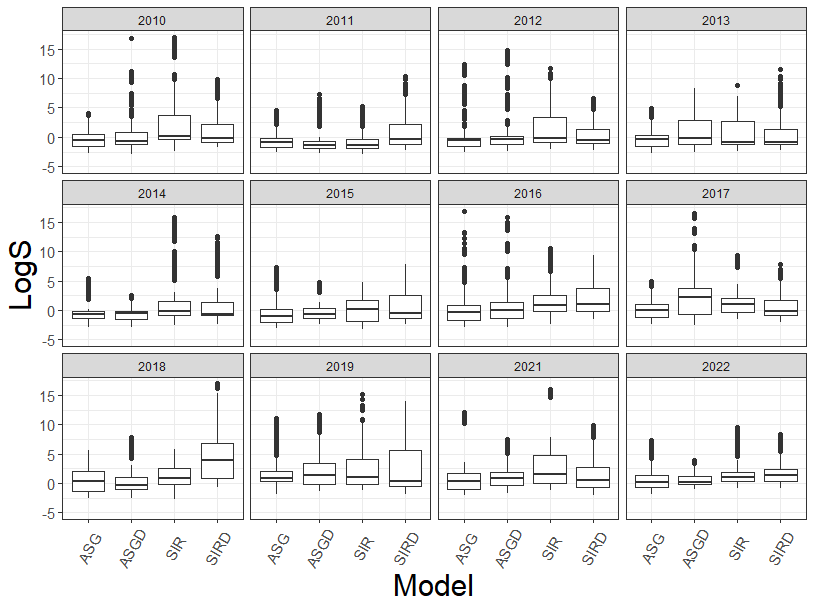
\includegraphics[scale=.5]{Images/logs_by_season.png}
    \caption{Boxplots of logarithmic score (LogS) for the four ILI models over all weeks and horizons in the simulation study faceted by season and including seasons 2010-2022, excluding 2020.}
    \label{fig:logs_by_season}
\end{figure}



% \section{Additional results plots for 2023-24 flu analysis}

In figure \ref{fig:lwis_by_traj_loc}, it appears that both the SIR and ASG models which include discrepancy perform slightly better than the models which do not.

\begin{figure}[hbt!]
    
    \centering
    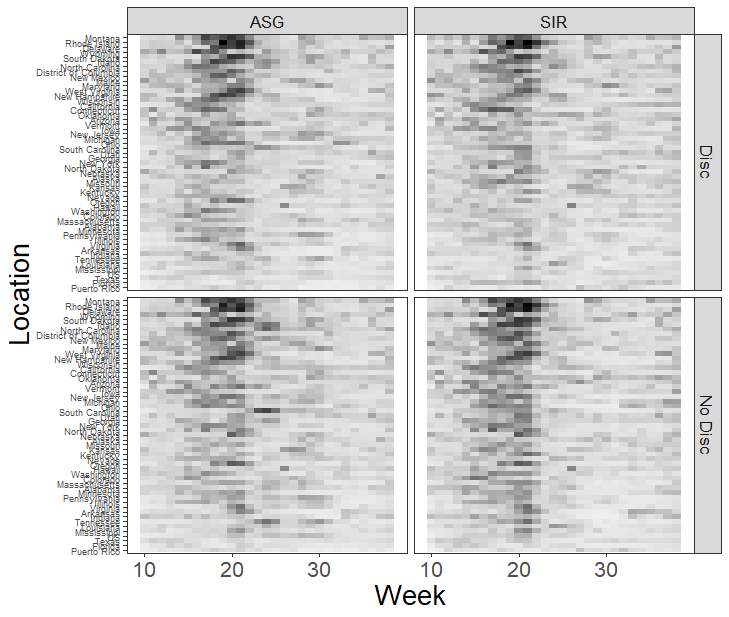
\includegraphics[scale = .7]{Images/lwis_by_traj_loc.png}
    \caption{Each plot shows the log weighted interval scores (LWIS) for all 50 US states, PR, DC, and national level forecasts at each week during the 2023 flu season. Scores are averaged over all horizons 1-4 weeks ahead. Scores are faceted by ILI model function (columns) and by whether or not discrepancy modeling was included (rows). The lighter the shade, the lower the LWIS with low LWIS being better.}
    \label{fig:lwis_by_traj_loc}
\end{figure}



\section{Posterior distribution plots for select parameters}
\label{app:B_prior}

The figures in this section show 95\% credible intervals for model parameters under the several modeling schemes along with the prior distributions assigned to the parameters. Figure \ref{fig:posterior_theta_sir} is for parameters unique to the SIR ILI model. Figures \ref{fig:posterior_theta} and \ref{fig:posterior_zeta} are for parameters unique to the ASG models. Figure \ref{fig:sir_asg_shared} is for parameters shared by SIR and ASG models, including parameters used for modeling discrepancy. Figures \ref{fig:hosp_lin_params} and \ref{fig:hosp_nus_param} are for parameters used in hospitalization modeling.


\begin{figure}[hbt!]
    \centering
    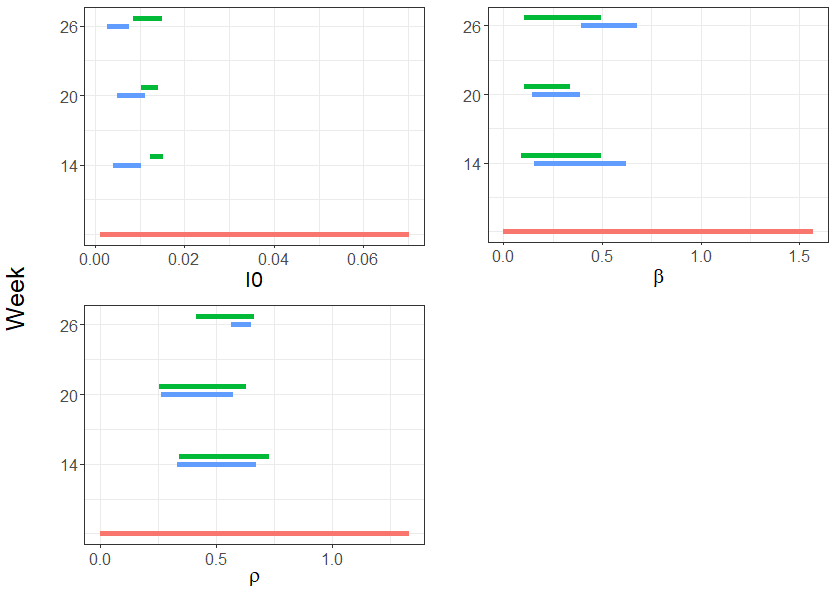
\includegraphics[scale=.6]{Images/posterior_theta_sir.png}
    \caption{Posterior 95\% credible intervals from ILI model for parameters of SIR differential equations. Shown are intervals from the US model of ILI for weeks 14, 20, and 26. The green is from the posterior where discrepancy is not modeled, and the blue is from the model where it is. The red interval is the 95\% interval of the prior distribution.}
    \label{fig:posterior_theta_sir}
\end{figure}

\begin{figure}[hbt!]
    \centering
    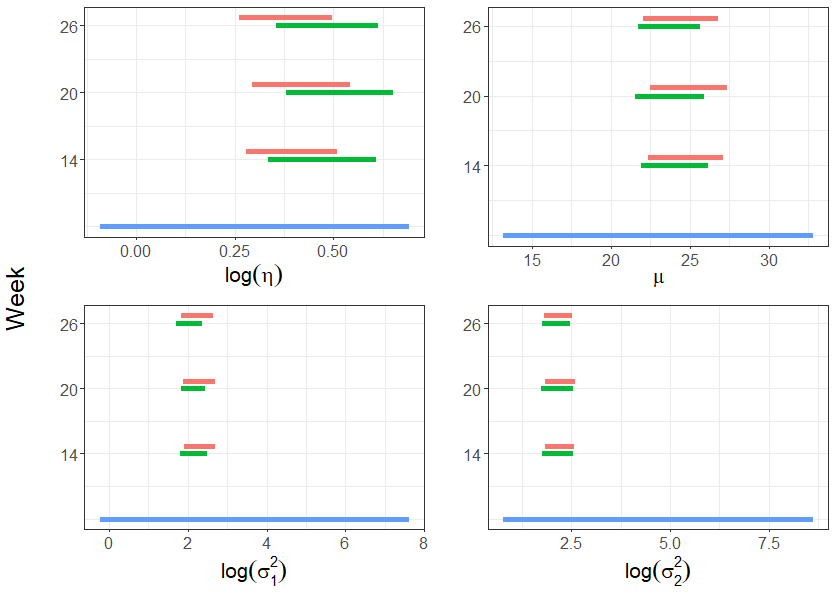
\includegraphics[scale=.6]{Images/posterior_theta.png}
    \caption{Posterior 95\% credible intervals from ILI model for parameters of ASG function. Shown are intervals from the US model of ILI for weeks 14, 20, and 26. The red is from the posterior where discrepancy is not modeled, and the green is from the model where it is. The blue interval is the 95\% interval of the prior distribution.}
    \label{fig:posterior_theta}
\end{figure}


\begin{figure}[hbt!]
    \centering
    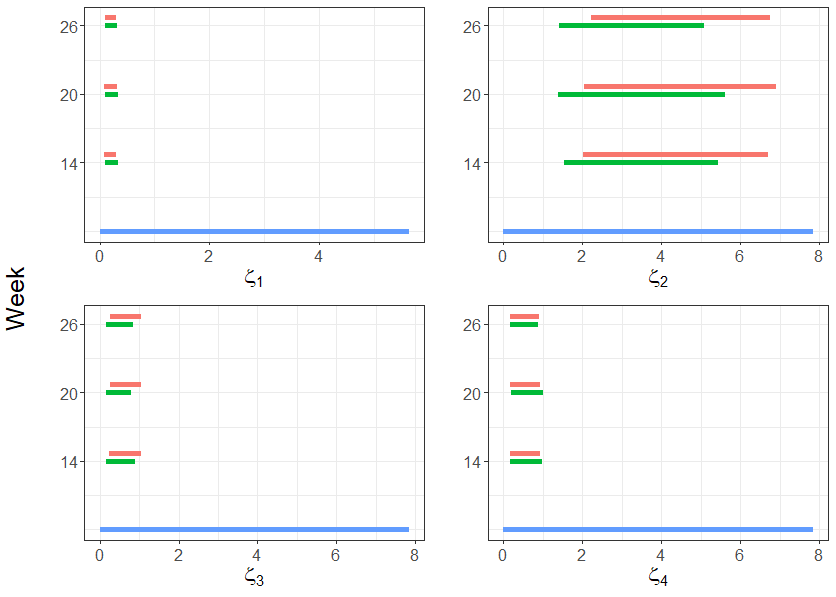
\includegraphics[scale=.6]{Images/posterior_zeta.png}
    \caption{Posterior 95\% credible intervals from ILI model for variance parameters of the ASG function. Shown are intervals from the US model of ILI for weeks 14, 20, and 26. The red is from the posterior where discrepancy is not modeled, and the green is from the model where it is. The blue interval is the 95\% interval of the prior distribution.}
    \label{fig:posterior_zeta}
\end{figure}

\begin{figure}[hbt!]
\centering
\begin{subfigure}
  \centering
  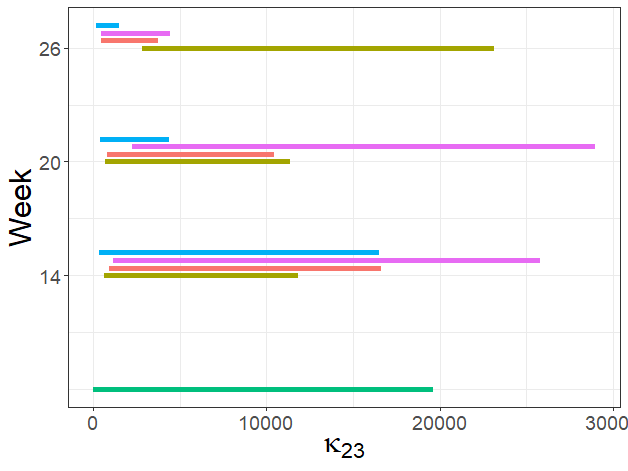
\includegraphics[width=.49\linewidth]{Images/posterior_kappa.png}
  % \caption{95\% posterior credible intervals from ILI model for scale parameter of the model distribution. Shown are intervals from the US model of ILI for weeks 14, 20, and 26. The blue is from the SIR model, purple from SIRD, red from ASG and yellow from ASGD. The green interval is the 95\% interval of the prior distribution.}
  % \label{fig:sub1}
\end{subfigure}%
\begin{subfigure}
  \centering
  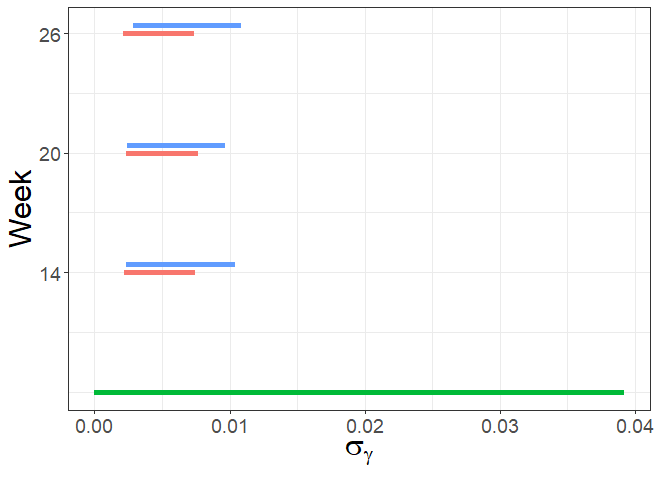
\includegraphics[width=.49\linewidth]{Images/posterior_sigma_gamma.png}
  % \caption{95\% posterior credible intervals from ILI model for scale parameter of modeled discrepancy. Shown are intervals from the US model of ILI for weeks 14, 20, and 26. The blue is from the SIRD model and red from ASGD. The green interval is the 95\% interval of the prior distribution.}
  % \label{fig:sub2}
\end{subfigure}
\caption{Posterior 95\% credible intervals from ILI model for scale parameter $\kappa_s$. Blue is from the SIR model, purple from SIRD, red from ASG and yellow from ASGD (left).  Posterior 95\% credible intervals from ILI model for scale parameter of modeled discrepancy $\sigma_{\gamma}$ (right). Shown are intervals from the US model of ILI for weeks 14, 20, and 26. Blue is from the SIRD model and red from ASGD. The green interval is the 95\% interval of the prior distribution.}
\label{fig:sir_asg_shared}
\end{figure}

% \begin{figure}[hbt!]
% 
% \begin{subfigure}
%   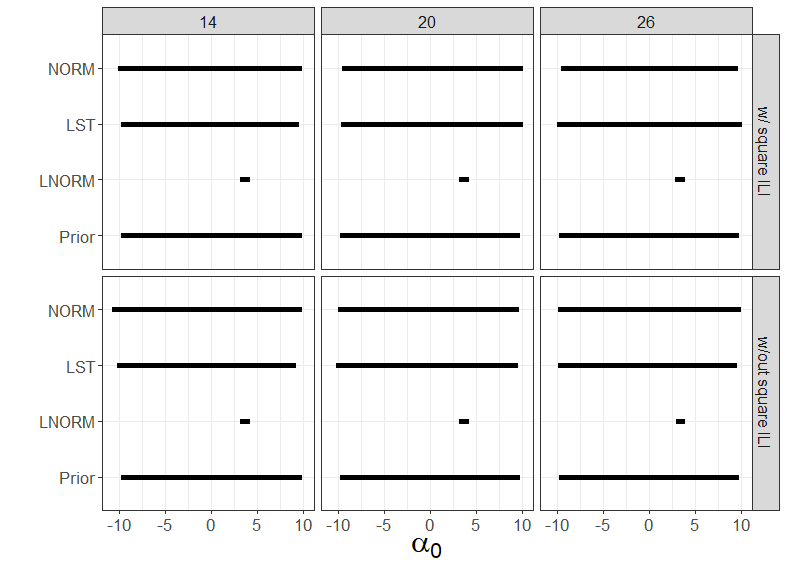
\includegraphics[width=.49\linewidth]{Images/alpha0_post.png}
%   % \caption{}
%   % \label{MLEDdet}
% \end{subfigure}\hfill % <-- "\hfill"
% \begin{subfigure}
%   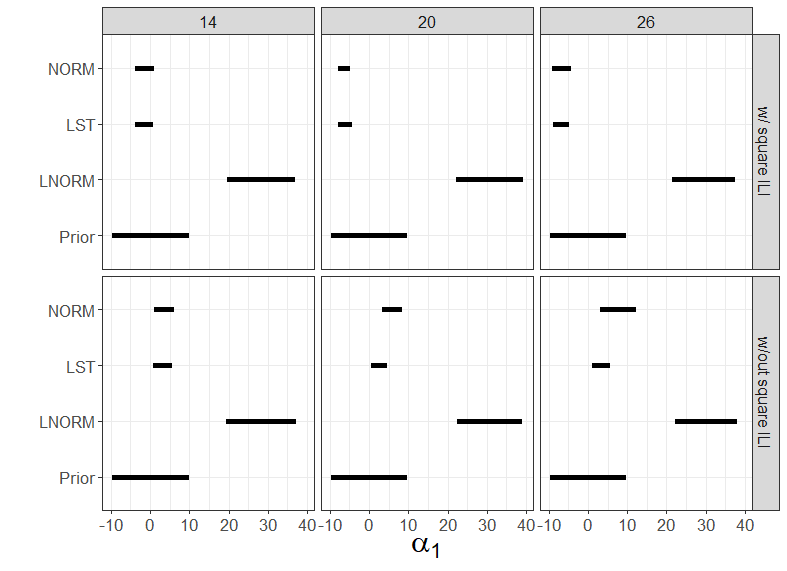
\includegraphics[width=.49\linewidth]{Images/alpha1_post.png}
%   % \caption{}
%   % \label{energydetPSK}
% \end{subfigure}
% 
% \medskip % create some *vertical* separation between the graphs
% \begin{subfigure}
%   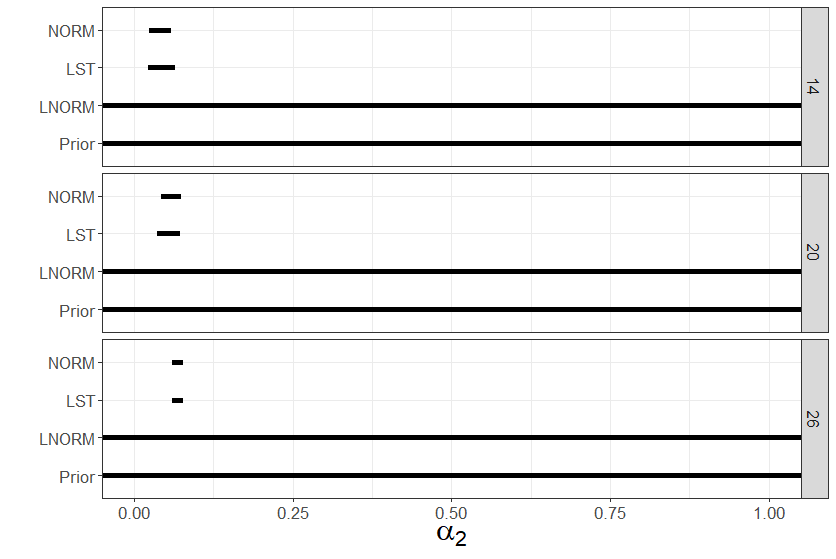
\includegraphics[width=.49\linewidth]{Images/alpha2_post.png}
%   % \caption{}
%   % \label{velcomp}
% \end{subfigure}\hfill % <-- "\hfill"
% \begin{subfigure}
%   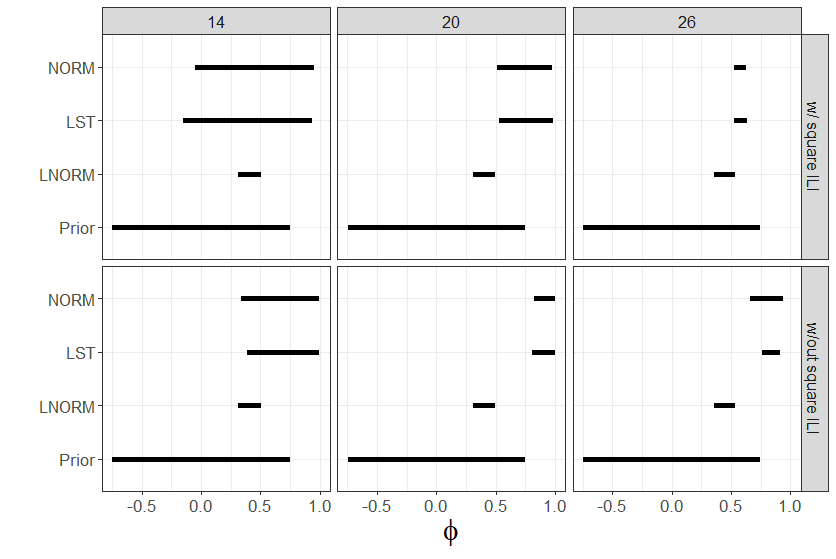
\includegraphics[width=.49\linewidth]{Images/phi_post.png}
%   % \caption{}
%   % \label{estcomp}
% \end{subfigure}






\begin{figure}[hbt!]
\centering
\begin{subfigure}
  \centering
  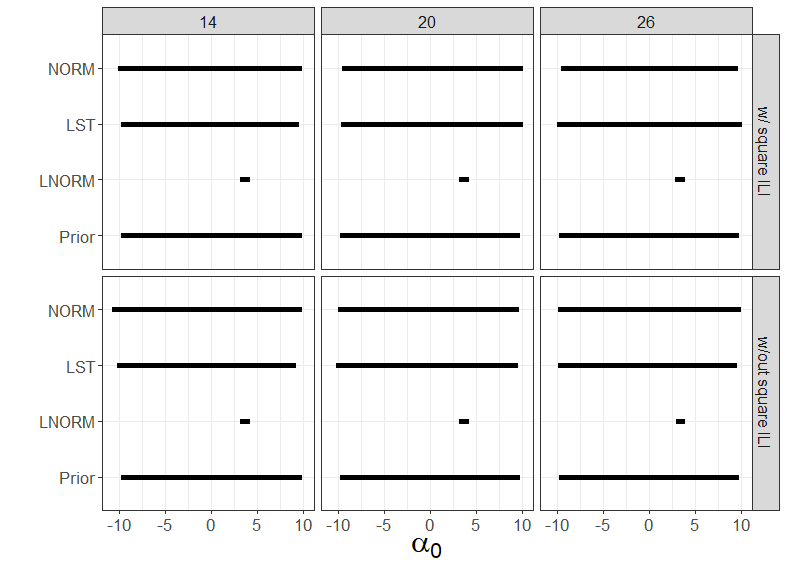
\includegraphics[width=.49\linewidth]{Images/alpha0_post.png}
\end{subfigure}%
\begin{subfigure}
  \centering
  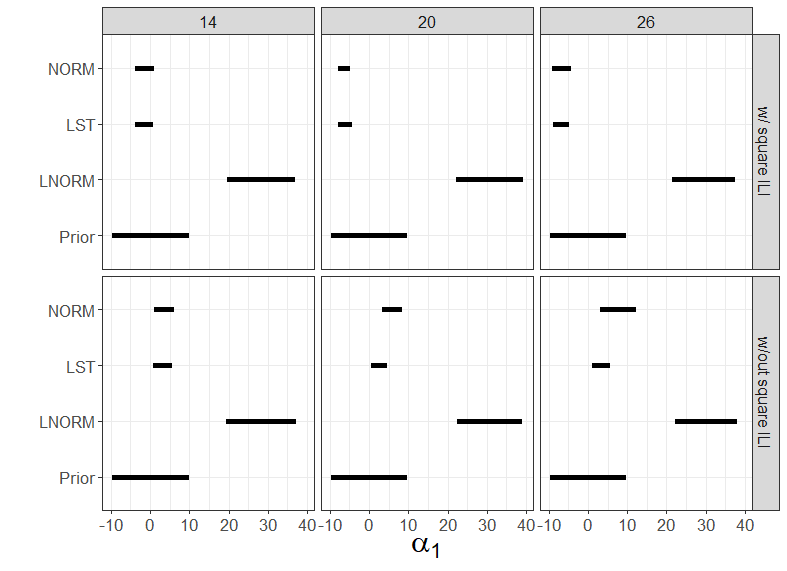
\includegraphics[width=.49\linewidth]{Images/alpha1_post.png}
\end{subfigure}
\begin{subfigure}
  \centering
  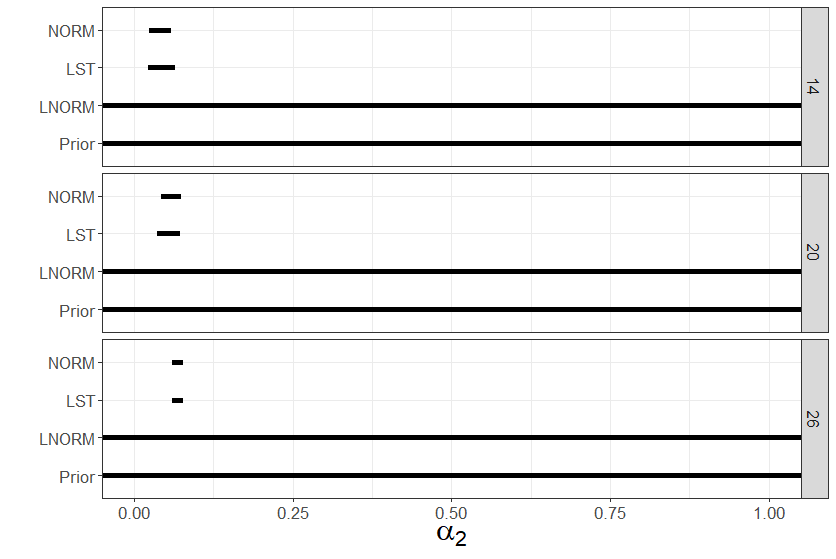
\includegraphics[width=.49\linewidth]{Images/alpha2_post.png}
\end{subfigure}%
\begin{subfigure}
  \centering
  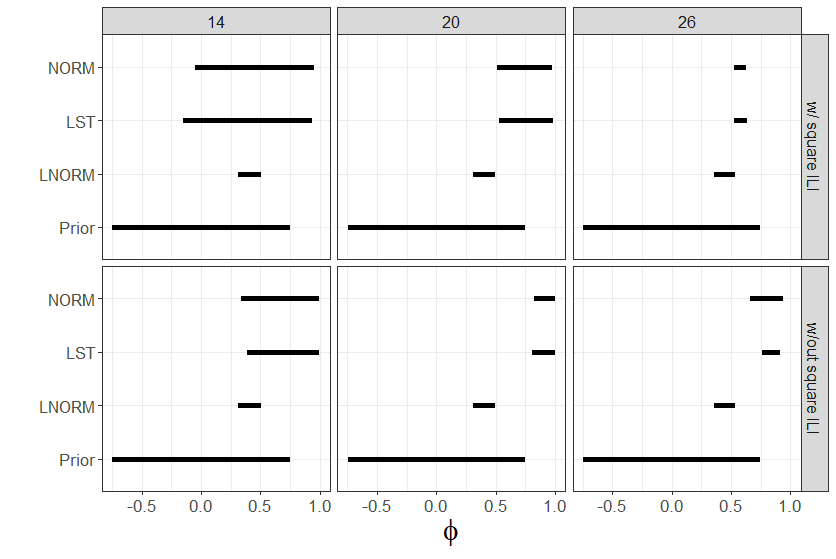
\includegraphics[width=.49\linewidth]{Images/phi_post.png}
\end{subfigure}
\caption{Posterior 95\% credible intervals for $\alpha_0$ for the three hospitalization models separated by whether or not the squared ILI term was included. Intervals are for the US hospitalizations and weeks 14, 20 and 26 are shown (top left). Prior distribution 95\% interval is also included.  95\% posterior credible intervals for $\alpha_1$ for the three hospitalization models separated by whether or not the squared ILI term was included. Intervals are for the US hospitalizations and weeks 14, 20 and 26 are shown (top right). Prior distribution 95\% interval is also included.
95\% posterior credible intervals for $\alpha_2$ for the three hospitalization models. Intervals are for the US hospitalizations and weeks 14, 20 and 26 are shown (bottom left). Prior distribution 95\% interval is also included. 
95\% posterior credible intervals for $\phi$ for the three hospitalization models separated by whether or not the squared ILI term was included (bottom right). Prior distribution 95\% interval is also included. In each plot intervals are for the US hospitalizations and weeks 14, 20 and 26 are shown.}
\label{fig:hosp_lin_params}
\end{figure}


% \begin{figure}[hbt!]
% 
% \begin{subfigure}
%   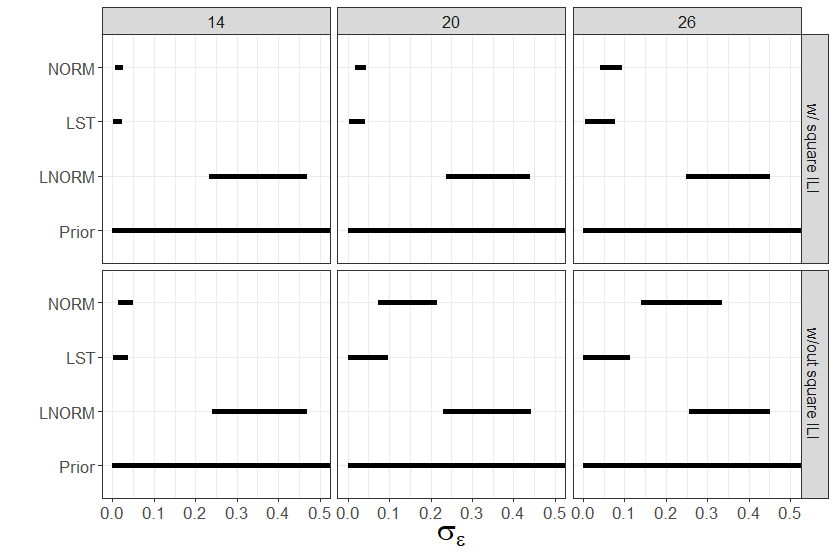
\includegraphics[width=\linewidth]{Images/sigma_epsilon_post.png}
%   % \caption{}
%   % \label{MLEDdet}
% \end{subfigure}\hfill % <-- "\hfill"
% \begin{subfigure}
%   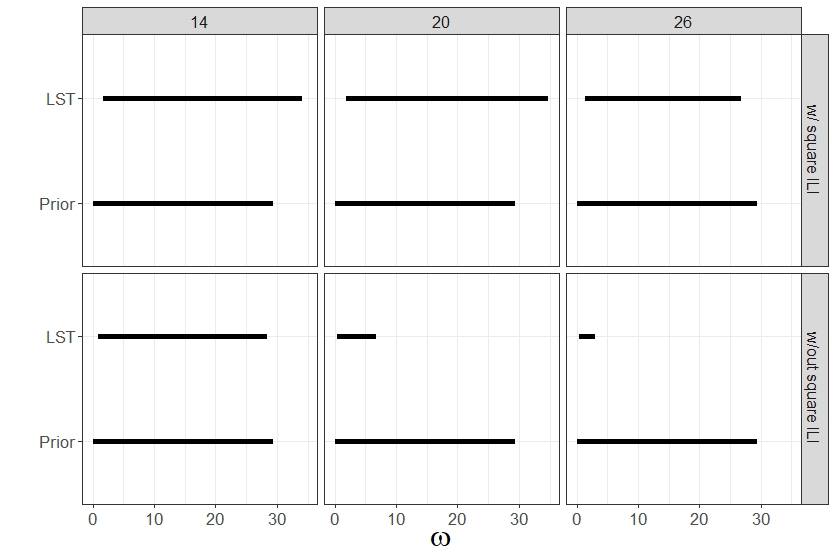
\includegraphics[width=\linewidth]{Images/omega_post.png}
%   % \caption{}
%   % \label{energydetPSK}
% \end{subfigure}
% 
% \caption{Posterior 95\% credible intervals for $\sigma_{\epsilon}$ for hospitalization models with and without the ILI squared term. Intervals are for the US hospitalizations and weeks 14, 20 and 26 are shown (left). Prior distribution 95\% interval is also included.
% 95\% posterior credible intervals for $\omega$ for LST hospitalization models with and without the ILI squared term (right). Prior distribution 95\% interval is also included. In all plots intervals are for the US hospitalizations and weeks 14, 20 and 26 are shown.}
% \label{fig:hosp_nus_param}
% \end{figure}




\begin{figure}[hbt!]
\centering
\begin{subfigure}
  \centering
  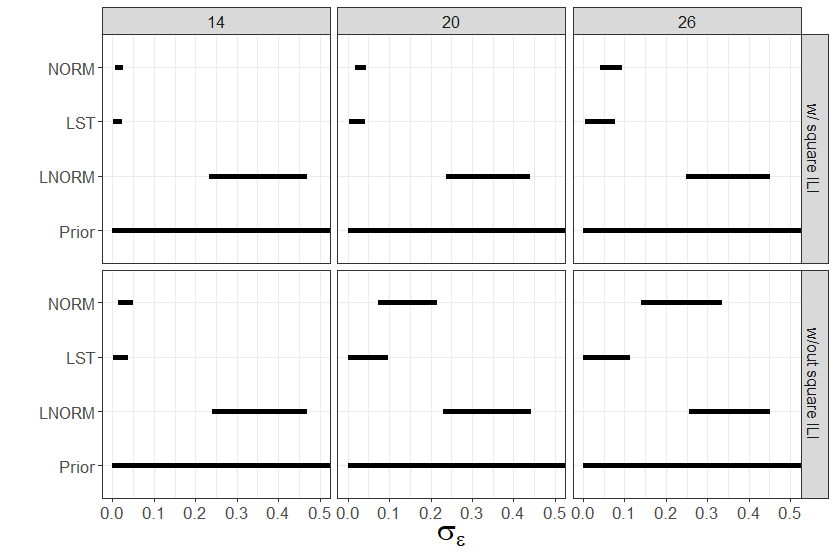
\includegraphics[width=.49\linewidth]{Images/sigma_epsilon_post.png}
  % \caption{95\% posterior credible intervals from ILI model for scale parameter of the model distribution. Shown are intervals from the US model of ILI for weeks 14, 20, and 26. The blue is from the SIR model, purple from SIRD, red from ASG and yellow from ASGD. The green interval is the 95\% interval of the prior distribution.}
  % \label{fig:sub1}
\end{subfigure}%
\begin{subfigure}
  \centering
  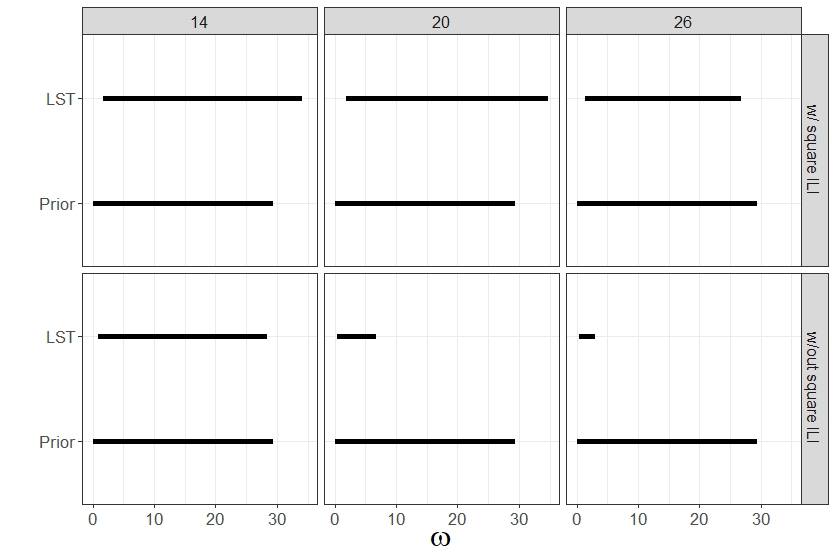
\includegraphics[width=.49\linewidth]{Images/omega_post.png}
  % \caption{95\% posterior credible intervals from ILI model for scale parameter of modeled discrepancy. Shown are intervals from the US model of ILI for weeks 14, 20, and 26. The blue is from the SIRD model and red from ASGD. The green interval is the 95\% interval of the prior distribution.}
  % \label{fig:sub2}
\end{subfigure}
\caption{Posterior 95\% credible intervals for $\sigma_{\epsilon}$ for hospitalization models with and without the ILI squared term. Intervals are for the US hospitalizations and weeks 14, 20 and 26 are shown (left). Prior distribution 95\% interval is also included.
95\% posterior credible intervals for $\omega$ for LST hospitalization models with and without the ILI squared term (right). Prior distribution 95\% interval is also included. In all plots intervals are for the US hospitalizations and weeks 14, 20 and 26 are shown.}
\label{fig:hosp_nus_param}
\end{figure}

\newpage
\section{FluSight forecast competition scoring results} \label{app:A_rwis}

In the CDC flu forecast competition, a baseline forecast was made to which all other forecasts were compared. The baseline forecast for a given state and week had as a median the most recent observed hospitalization count. The uncertainty was based on differences between previous hospitalizations, and is similar to the baseline forecast used in previous flu forecasting seasons and in the COVID-19 hub \cite[]{mathis2024evaluation, cramer2022evaluation}. 
The RWIS for one model was calculated by first taking the ratio of the average LWIS paired with every other model. This was then diveded by the same ratio for the baseline forecasts (see methods in \cite{mathis2024evaluation} for details).
 An RWIS less than 1 indicates the forecast outperformed the baseline forecast.
 Figures \ref{fig:rwis_ili_tile} and \ref{fig:rwis_hosp_tile} show the mean RWIS of hospitalization forecasts over all 24 models from the main manuscript for all locations and weeks of the 2023 flu season. Some similar patterns to those noted in section the manuscript emerge, including a slightly better performance by forecasts including discrepancy modeling over those which do not include discrepancy modeling and better overall performance by the SIR models than by the ASG forecast models. Interestingly, figure \ref{fig:rwis_hosp_tile} shows the LNORM model showing especially poor RWIS performance about three quarters into the season. This was not seen in the LWIS in the main manuscript. %figure \ref{fig:lwis_by_dist_loc}. 


\begin{figure}[hbt!]
    \centering
    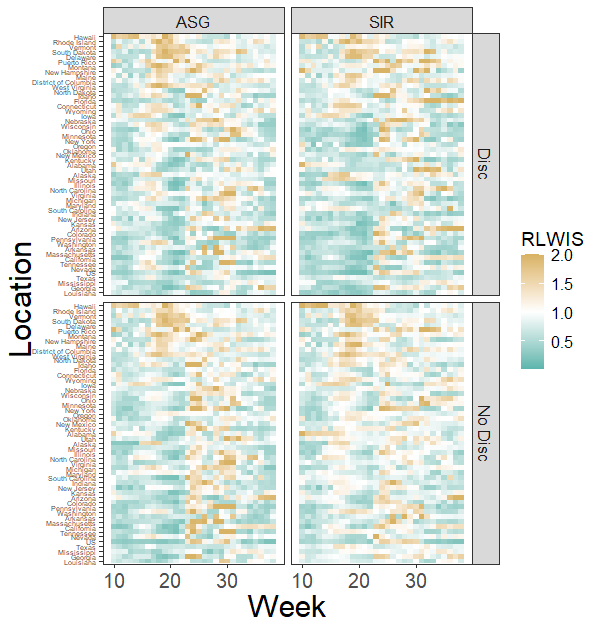
\includegraphics[scale=.7]{Images/rwis_ili_mod.png}
    \caption{RWIS averaged over all 24 models and horizons for forecasts across all locations and weeks. The plot is separated by the four ILI models. Dark blue is lower RWIS, and dark tan is higher RWIS where white is RWIS = 1}
    \label{fig:rwis_ili_tile}
\end{figure}


\begin{figure}[hbt!]
    \centering
    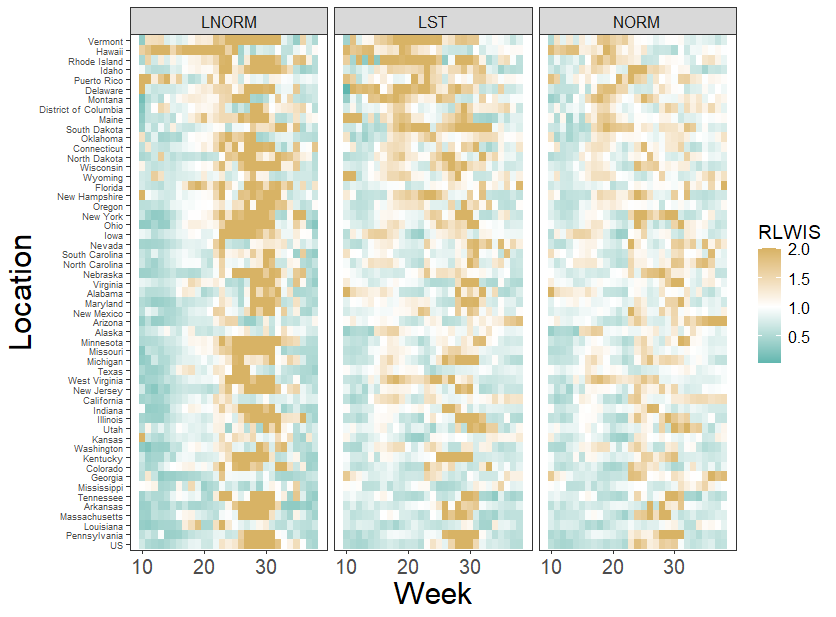
\includegraphics[scale=.6]{Images/rwis_hosp_mod.png}
    \caption{RWIS averaged over all 24 models and horizons for forecasts across all locations and weeks. The plot is separated by the three distribution choices for the hospitalization model. Dark blue is lower RWIS, and dark tan is higher RWIS where white is RWIS = 1}
    \label{fig:rwis_hosp_tile}
\end{figure}


Figure \ref{fig:state_median_points} shows the mean over weeks RWIS for the SIR and ASG forecast models with an RWIS less than 1 for the most locations. The plot on the left is from a forecast by an SIRD ILI model and a quadratic NORM hospitalization model. This forecast model had an RWIS less than 1 for 37 out of 53 locations. The plot on the right is from a forecast by an ASGD ILI model and linear NORM hospitalization model. This model had an RWIS less than 1 for 34 out of 53 locations.

\begin{figure}[hbt!]
\centering
\begin{subfigure}
  \centering
  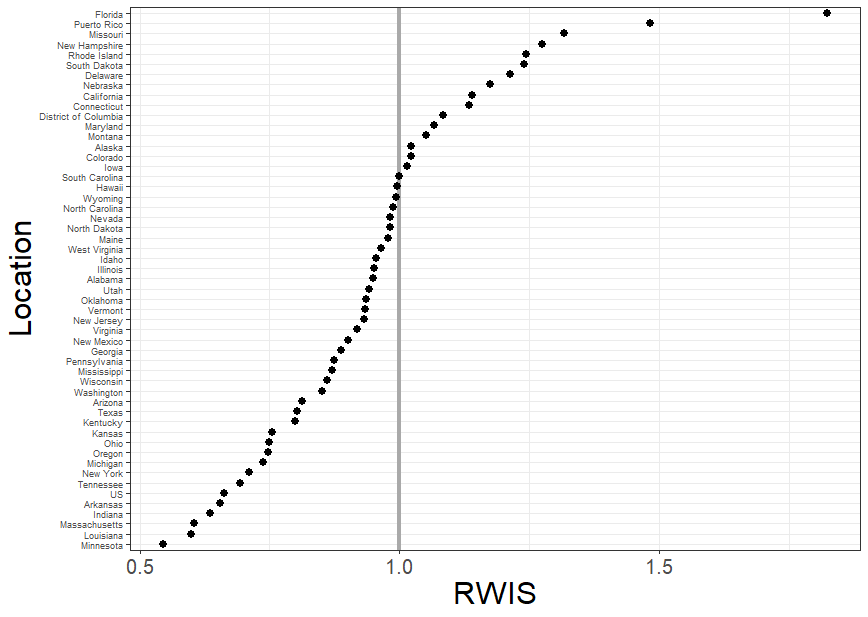
\includegraphics[width=.49\linewidth]{Images/sir_disc_hosp_sq_ar1_rwis.png}
  % \caption{A subfigure}
  % \label{fig:sub1}
\end{subfigure}%
\begin{subfigure}
  \centering
  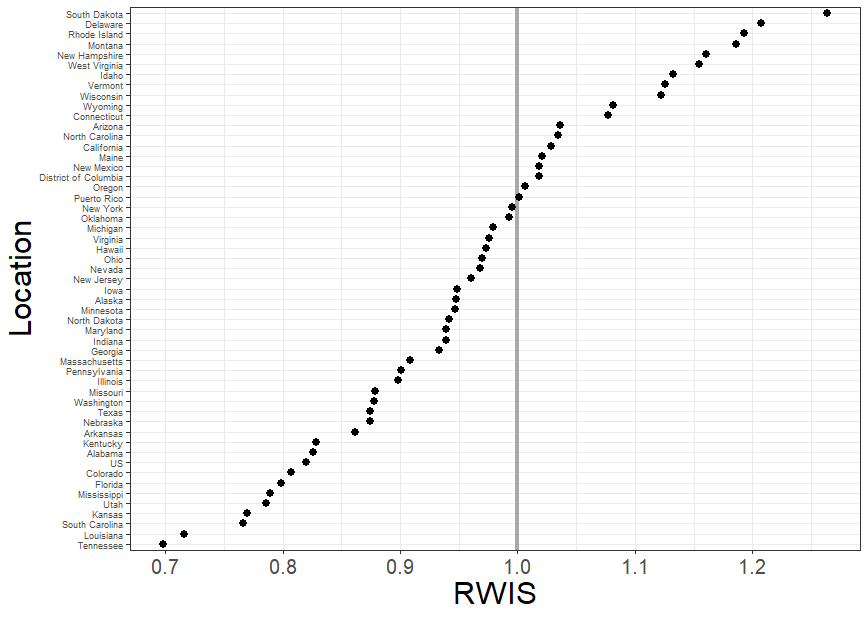
\includegraphics[width=.49\linewidth]{Images/asg_disc_hosp_ar1_rwis.png}
  % \caption{A subfigure}
  % \label{fig:sub2}
\end{subfigure}
\caption{RWIS over the whole 2023 flu season for all 53 locations for hospitalization forecasts from an SIRD quadratic hospitalization model with normal errors (left) and forecasts from an ASGD linear hospitalization model with normal errors (right). An RWIS less than 1 (left of vertical grey line) indicates the model forecasts outperformed the baseline forecasts for that particular region.}
\label{fig:state_median_points}
\end{figure}
\end{supplement}






\bibliographystyle{ba}
\bibliography{master_bib}

\end{document}

